% !TEX TS-program = pdflatex
\documentclass[11pt]{article}

% -------------------- Packages --------------------
\usepackage[a4paper,margin=1in]{geometry}
\usepackage{amsmath,amssymb}
\usepackage[T1]{fontenc}
\usepackage{lmodern}
\usepackage{xcolor}
\usepackage{tcolorbox}
\tcbuselibrary{skins,breakable}
\usepackage{enumitem}
\usepackage{hyperref}
\usepackage{tikz}
\usetikzlibrary{calc,angles,quotes,arrows.meta}

\pagestyle{empty}

% -------------------- Dark Theme Colors --------------------
\definecolor{bg}{HTML}{000000}
\definecolor{pairbg}{HTML}{121212}
\definecolor{solbg}{HTML}{0A0A0A}
\definecolor{border}{HTML}{2A2A2A}
\definecolor{text}{HTML}{FFFFFF}
\definecolor{muted}{HTML}{C9CDD3}
\definecolor{gold}{HTML}{FFD700}
\definecolor{green}{HTML}{4ADE80}
\definecolor{cyan}{HTML}{38BDF8}

\pagecolor{bg}
\color{text}

\hypersetup{
  colorlinks=true,
  linkcolor=cyan,
  urlcolor=cyan
}

\setlength{\parindent}{0pt}
\setlength{\parskip}{10pt}

% Help LaTeX avoid overfull lines globally
\sloppy
\setlength{\emergencystretch}{3em}

\setlist[itemize]{left=1.4em,itemsep=6pt,topsep=6pt}
\setlist[enumerate]{left=1.6em,itemsep=4pt,topsep=4pt}

% -------------------- tcolorbox Base --------------------
\tcbset{
  enhanced,
  breakable,
  arc=12pt,
  boxrule=0.8pt,
  left=14pt,right=14pt,top=12pt,bottom=12pt
}

\newtcolorbox{QAPair}[1]{%
  colback=pairbg,
  colbacklower=solbg,
  colframe=border,
  coltext=text,
  title=\textcolor{gold}{\bfseries #1},
  fonttitle=\bfseries,
  coltitle=text,
  segmentation style={draw=border, dashed, line width=0.6pt},
  before upper=\raggedright,
  before lower=\raggedright
}

\newtcolorbox{QuickBox}{%
  colback=pairbg,
  colframe=cyan,
  coltext=text,
  fontupper=\color{text}\raggedright,
  borderline north={4pt}{0pt}{cyan},
  arc=14pt,
  boxrule=0.8pt
}

% Helper for step headings
\newcommand{\Step}[1]{\textcolor{muted}{\textbf{Step #1:}}}

% Small centered diagram block (for step-by-step visuals)
\newenvironment{StepDiagram}{\par\medskip\begin{center}}{\end{center}\medskip}

% TikZ styles
\tikzset{
  base/.style={draw=text, line width=0.9pt, line cap=round, line join=round},
  new/.style={draw=cyan, line width=1.2pt, line cap=round, line join=round},
  help/.style={draw=muted, dashed, line width=0.9pt},
  ang/.style={draw=gold, line width=1.0pt},
  dot/.style={circle, fill=text, inner sep=1.2pt},
  lab/.style={text=text, font=\small},
  labm/.style={text=muted, font=\small},
}

% A tiny "equation diagram" (counts as a step-visual)
\newcommand{\EqDiagram}[1]{%
\begin{StepDiagram}
\begin{tikzpicture}
\node[draw=border, rounded corners=10pt, inner sep=8pt, text=text, align=left, text width=0.88\linewidth] {#1};
\end{tikzpicture}
\end{StepDiagram}
}

% ============================================================
\begin{document}

\begin{center}
{\LARGE\bfseries \textcolor{gold}{Exercise 9.4 --- Solutions}}\\[-2pt]
\end{center}

% -------------------- Quick formulas + DIAGRAMS --------------------
\begin{QuickBox}
{\color{cyan}\bfseries Quick formulas (Arcs \& Sectors)}\par\medskip

\begin{itemize}
\item \textbf{Circumference:} $C=2\pi r$.

\item \textbf{Arc length (central angle $\theta^\circ$):}
\[
s=\frac{\theta}{360^\circ}\,(2\pi r).
\]
\begin{StepDiagram}
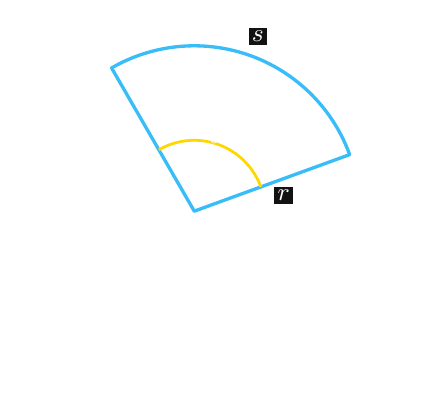
\begin{tikzpicture}[scale=1.05]
  \def\r{2.0}
  \def\angA{20}
  \def\angB{120}
  \coordinate (O) at (0,0);
  \coordinate (A) at (\angA:\r);
  \coordinate (B) at (\angB:\r);

  \draw[base] (O) circle (\r);
  \node[dot,label={[lab]below:$O$}] at (O) {};
  \node[dot,label={[lab]right:$A$}] at (A) {};
  \node[dot,label={[lab]left:$B$}] at (B) {};

  \draw[new] (O)--(A);
  \draw[new] (O)--(B);

  % arc highlight
  \draw[new] (\angA:\r) arc (\angA:\angB:\r);
  \node[lab, fill=pairbg, inner sep=1.2pt] at (70:2.25) {$s$};

  \pic[ang,"$\theta^\circ$",lab,angle radius=9mm,angle eccentricity=1.15] {angle=A--O--B};
  \node[lab, fill=pairbg, inner sep=1.2pt] at (10:1.1) {$r$};
\end{tikzpicture}
\end{StepDiagram}

\item \textbf{Area of sector:}
\[
A_{\text{sector}}=\frac{\theta}{360^\circ}\,\pi r^2.
\]
\begin{StepDiagram}
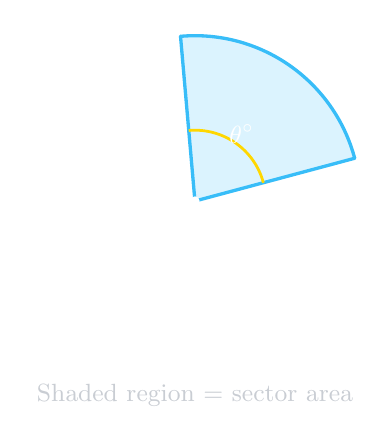
\begin{tikzpicture}[scale=1.05]
  \def\r{2.0}
  \def\angA{15}
  \def\angB{95}
  \coordinate (O) at (0,0);
  \coordinate (A) at (\angA:\r);
  \coordinate (B) at (\angB:\r);

  \draw[base] (O) circle (\r);
  \fill[cyan, opacity=0.18] (O)--(A) arc (\angA:\angB:\r)--cycle;

  \draw[new] (O)--(A);
  \draw[new] (O)--(B);
  \draw[new] (A) arc (\angA:\angB:\r);

  \node[dot,label={[lab]below:$O$}] at (O) {};
  \pic[ang,"$\theta^\circ$",lab,angle radius=9mm,angle eccentricity=1.15] {angle=A--O--B};
  \node[labm] at (0,-2.35) {Shaded region = sector area};
\end{tikzpicture}
\end{StepDiagram}

\item \textbf{Chord length (central angle $\theta$):}
\[
c=2r\sin\!\left(\frac{\theta}{2}\right).
\]
\begin{StepDiagram}
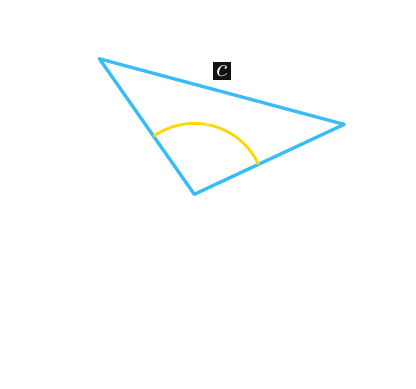
\begin{tikzpicture}[scale=1.05]
  \def\r{2.0}
  \def\angA{25}
  \def\angB{125}
  \coordinate (O) at (0,0);
  \coordinate (A) at (\angA:\r);
  \coordinate (B) at (\angB:\r);

  \draw[base] (O) circle (\r);
  \node[dot,label={[lab]below:$O$}] at (O) {};
  \node[dot,label={[lab]right:$A$}] at (A) {};
  \node[dot,label={[lab]left:$B$}] at (B) {};

  \draw[new] (O)--(A);
  \draw[new] (O)--(B);
  \draw[new] (A)--(B);
  \node[lab, fill=pairbg, inner sep=1.2pt] at ($(A)!0.5!(B)+(0,0.25)$) {$c$};

  \pic[ang,"$\theta^\circ$",lab,angle radius=9mm,angle eccentricity=1.15] {angle=A--O--B};
\end{tikzpicture}
\end{StepDiagram}

\item \textbf{Area of segment (minor):}
\[
A_{\text{seg}}=A_{\text{sector}}-A_{\triangle}
=\frac{\theta}{360^\circ}\pi r^2-\frac12 r^2\sin\theta.
\]
\begin{StepDiagram}
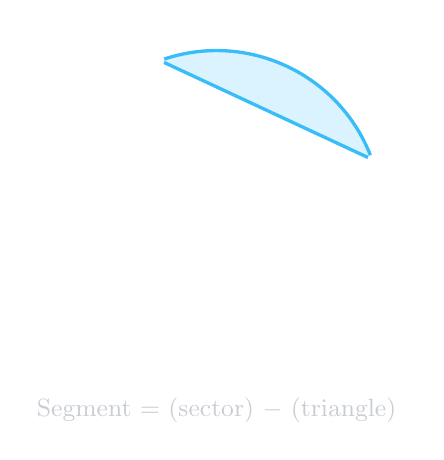
\begin{tikzpicture}[scale=1.05]
  \def\r{2.0}
  \def\angA{20}
  \def\angB{110}
  \coordinate (O) at (0,0);
  \coordinate (A) at (\angA:\r);
  \coordinate (B) at (\angB:\r);

  \draw[base] (O) circle (\r);
  \fill[cyan, opacity=0.18] (A) arc (\angA:\angB:\r)--(B)--cycle; % segment fill (approx)
  \draw[new] (A)--(B);
  \draw[new] (\angA:\r) arc (\angA:\angB:\r);

  \node[dot,label={[lab]below:$O$}] at (O) {};
  \node[dot,label={[lab]right:$A$}] at (A) {};
  \node[dot,label={[lab]left:$B$}] at (B) {};
  \node[labm] at (0,-2.35) {Segment = (sector) $-$ (triangle)};
\end{tikzpicture}
\end{StepDiagram}
\end{itemize}
\end{QuickBox}

% ============================================================
% Q1
\begin{QAPair}{Question 1}
\textcolor{gold}{\bfseries Question:} In the figure, radius of circle is $7$ cm. Find: \\
(i) the length of minor arc $\overset{\frown}{PQ}$ and major arc $\overset{\frown}{PAQ}$. \\
(ii) the circumference of circle. \\
Is the sum of lengths of minor arc and major arc equal to the circumference of circle?
\tcblower
\textcolor{green}{\bfseries Answer:}\par

\Step{1} Mark the central angle $\angle POQ=100^\circ$ and radius $r=7$ cm.
\begin{StepDiagram}
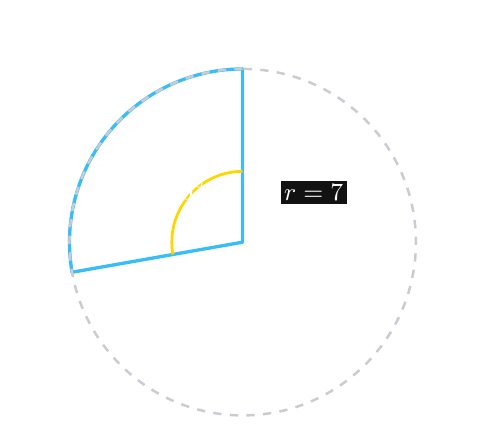
\begin{tikzpicture}[scale=1.0]
  \def\r{2.2}
  \coordinate (O) at (0,0);
  \coordinate (P) at (90:\r);
  \coordinate (Q) at (190:\r);
  \coordinate (A) at (0:\r);

  \draw[base] (O) circle (\r);
  \node[dot,label={[lab]below:$O$}] at (O) {};
  \node[dot,label={[lab]above:$P$}] at (P) {};
  \node[dot,label={[lab]left:$Q$}] at (Q) {};
  \node[dot,label={[lab]right:$A$}] at (A) {};

  \draw[new] (O)--(P);
  \draw[new] (O)--(Q);

  \draw[new] (P) arc (90:190:\r); % minor arc PQ
  \draw[help] (P) arc (90:450:\r); % faint whole circle sweep reference

  \pic[ang,"$100^\circ$",lab,angle radius=9mm,angle eccentricity=1.15] {angle=P--O--Q};
  \node[lab, fill=pairbg, inner sep=1.2pt] at (35:1.1) {$r=7$};
\end{tikzpicture}
\end{StepDiagram}

\Step{2} Circumference:
\[
C=2\pi r=2\pi(7)=14\pi\ \text{cm}.
\]
\EqDiagram{$C=2\pi(7)=14\pi\ \text{cm}$}

\Step{3} Minor arc $\overset{\frown}{PQ}$ corresponds to $100^\circ$:
\[
\ell(\overset{\frown}{PQ})=\frac{100}{360}\cdot 14\pi=\frac{35}{9}\pi\ \text{cm}.
\]
\EqDiagram{$\ell(\overset{\frown}{PQ})=\dfrac{100}{360}\cdot 14\pi=\dfrac{35}{9}\pi\ \text{cm}$}

\Step{4} Major arc $\overset{\frown}{PAQ}$ is the rest of the circle:
\[
\ell(\overset{\frown}{PAQ})=C-\ell(\overset{\frown}{PQ})
=14\pi-\frac{35}{9}\pi=\frac{91}{9}\pi\ \text{cm}.
\]
\begin{StepDiagram}
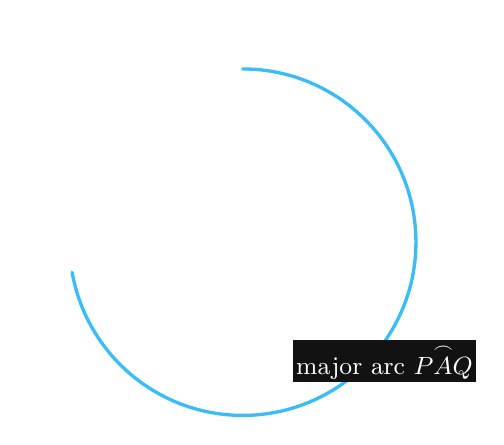
\begin{tikzpicture}[scale=1.0]
  \def\r{2.2}
  \coordinate (O) at (0,0);
  \coordinate (P) at (90:\r);
  \coordinate (Q) at (190:\r);
  \coordinate (A) at (0:\r);

  \draw[base] (O) circle (\r);
  \node[dot,label={[lab]below:$O$}] at (O) {};
  \node[dot,label={[lab]above:$P$}] at (P) {};
  \node[dot,label={[lab]left:$Q$}] at (Q) {};
  \node[dot,label={[lab]right:$A$}] at (A) {};

  \draw[new] (P) arc (90:-170:\r); % major arc from P to Q passing A
  \node[lab, fill=pairbg, inner sep=1.2pt] at (-40:2.35) {major arc $\overset{\frown}{PAQ}$};
\end{tikzpicture}
\end{StepDiagram}

\Step{5} Check:
\[
\ell(\overset{\frown}{PQ})+\ell(\overset{\frown}{PAQ})
=\frac{35}{9}\pi+\frac{91}{9}\pi=14\pi=C.
\]
\EqDiagram{Yes. Minor + major $=14\pi=C$}

\[
\boxed{\ell(\overset{\frown}{PQ})=\frac{35}{9}\pi\ \text{cm},\quad
\ell(\overset{\frown}{PAQ})=\frac{91}{9}\pi\ \text{cm},\quad
C=14\pi\ \text{cm}.}
\]
\end{QAPair}

% ============================================================
% Q2
\begin{QAPair}{Question 2}
\textcolor{gold}{\bfseries Question:} Given the radius of circle is $8$ cm. Find: \\
(i) the area of minor sector and major sector. \\
(ii) the area of circle. \\
Is the sum of areas of minor and major sectors equal to the area of circle?
\tcblower
\textcolor{green}{\bfseries Answer:}\par

\Step{1} From the figure, the central angle of the minor sector is $60^\circ$ and $r=8$ cm.
\begin{StepDiagram}
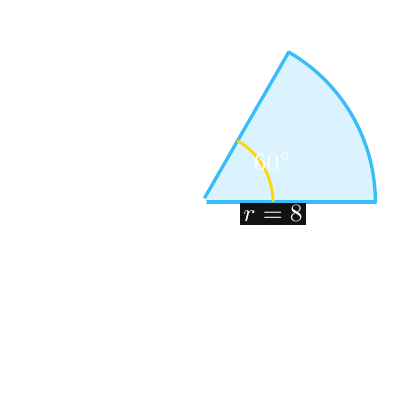
\begin{tikzpicture}[scale=1.0]
  \def\r{2.2}
  \def\a{0}
  \def\b{60}
  \coordinate (O) at (0,0);
  \coordinate (A) at (\a:\r);
  \coordinate (B) at (\b:\r);

  \draw[base] (O) circle (\r);
  \fill[cyan, opacity=0.18] (O)--(A) arc (\a:\b:\r)--cycle;
  \draw[new] (O)--(A);
  \draw[new] (O)--(B);
  \draw[new] (A) arc (\a:\b:\r);

  \node[dot,label={[lab]below:$O$}] at (O) {};
  \pic[ang,"$60^\circ$",lab,angle radius=9mm,angle eccentricity=1.15] {angle=A--O--B};
  \node[lab, fill=pairbg, inner sep=1.2pt] at (0.9,-0.15) {$r=8$};
\end{tikzpicture}
\end{StepDiagram}

\Step{2} Area of circle:
\[
A_{\text{circle}}=\pi r^2=\pi(8^2)=64\pi\ \text{cm}^2.
\]
\EqDiagram{$A_{\text{circle}}=\pi(8^2)=64\pi\ \text{cm}^2$}

\Step{3} Area of minor sector ($60^\circ$):
\[
A_{\text{minor}}=\frac{60}{360}\cdot 64\pi=\frac{32}{3}\pi\ \text{cm}^2.
\]
\EqDiagram{$A_{\text{minor}}=\dfrac{60}{360}\cdot 64\pi=\dfrac{32}{3}\pi\ \text{cm}^2$}

\Step{4} Area of major sector:
\[
A_{\text{major}}=A_{\text{circle}}-A_{\text{minor}}
=64\pi-\frac{32}{3}\pi=\frac{160}{3}\pi\ \text{cm}^2.
\]
\EqDiagram{$A_{\text{major}}=64\pi-\dfrac{32}{3}\pi=\dfrac{160}{3}\pi\ \text{cm}^2$}

\Step{5} Check:
\[
A_{\text{minor}}+A_{\text{major}}=\frac{32}{3}\pi+\frac{160}{3}\pi=64\pi=A_{\text{circle}}.
\]
\EqDiagram{Yes. Minor + major $=64\pi$}

\[
\boxed{A_{\text{minor}}=\frac{32}{3}\pi,\quad
A_{\text{major}}=\frac{160}{3}\pi,\quad
A_{\text{circle}}=64\pi\ \text{cm}^2.}
\]
\end{QAPair}

% ============================================================
% Q3
\begin{QAPair}{Question 3}
\textcolor{gold}{\bfseries Question:} Find the distance covered by the tip of hour hand of a clock in $5$ hours if the length of hour hand is $10$ cm.
\tcblower
\textcolor{green}{\bfseries Answer:}\par

\Step{1} In $12$ hours, the hour hand makes $360^\circ$. In $5$ hours it makes
\[
\theta=\frac{5}{12}\cdot 360^\circ=150^\circ.
\]
\begin{StepDiagram}
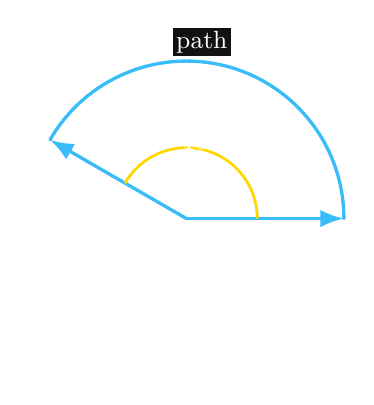
\begin{tikzpicture}[scale=1.0]
  \def\r{2.0}
  \def\a{0}
  \def\b{150}
  \coordinate (O) at (0,0);
  \coordinate (H1) at (\a:\r);
  \coordinate (H2) at (\b:\r);

  \draw[base] (O) circle (\r);
  \node[dot,label={[lab]below:$O$}] at (O) {};
  \draw[new, -{Latex[length=3mm]}] (O)--(H1);
  \draw[new, -{Latex[length=3mm]}] (O)--(H2);

  \draw[new] (H1) arc (\a:\b:\r);
  \node[lab, fill=pairbg, inner sep=1.2pt] at (85:2.25) {path};

  \pic[ang,"$150^\circ$",lab,angle radius=9mm,angle eccentricity=1.15] {angle=H1--O--H2};
\end{tikzpicture}
\end{StepDiagram}

\Step{2} The tip moves on a circle of radius $r=10$ cm, so distance (arc length) is
\[
s=\frac{150}{360}\cdot 2\pi(10)=\frac{25}{3}\pi\ \text{cm}.
\]
\EqDiagram{$s=\dfrac{150}{360}\cdot 2\pi(10)=\dfrac{25}{3}\pi\ \text{cm}\ (\approx 26.18\text{ cm})$}

\[
\boxed{s=\frac{25}{3}\pi\ \text{cm}}
\]
\end{QAPair}

% ============================================================
% Q4
\begin{QAPair}{Question 4}
\textcolor{gold}{\bfseries Question:} Given the sector of circle (as shown). Find: \\
(i) length of outer minor arc,\;
(ii) length of inner minor arc,\;
(iii) difference of lengths,\;
(iv) area of minor sector of bigger circle,\;
(v) area of minor sector of smaller circle,\;
(vi) area of shaded part.
\tcblower
\textcolor{green}{\bfseries Answer:}\par

\Step{1} From the figure: central angle $60^\circ$, outer radius $R=21$ cm, inner radius $r=10$ cm.
\begin{StepDiagram}
\begin{tikzpicture}[scale=1.0]
  \def\R{2.2}
  \def\r{1.05}
  \def\a{0}
  \def\b{60}
  \coordinate (O) at (0,0);

  % annular sector fill (shaded part)
  \fill[cyan, opacity=0.18] (O) ++(\a:\R) arc (\a:\b:\R) -- ++(\b:\r-\R)
    arc (\b:\a:\r) -- cycle;

  % circles (just arcs)
  \draw[base] (O) circle (\R);
  \draw[base] (O) circle (\r);

  % radii
  \draw[new] (O)--(\a:\R);
  \draw[new] (O)--(\b:\R);

  \node[dot,label={[lab]below:$O$}] at (O) {};
  \pic[ang,"$60^\circ$",lab,angle radius=9mm,angle eccentricity=1.15] {angle={(\a:\R)}--O--{(\b:\R)}};

  \node[labm] at (0,-2.55) {Outer radius $=21$, inner radius $=10$ (same centre)};
\end{tikzpicture}
\end{StepDiagram}

\Step{2} Outer minor arc:
\[
\ell_{\text{outer}}=\frac{60}{360}\cdot 2\pi(21)=7\pi\ \text{cm}.
\]
\EqDiagram{$\ell_{\text{outer}}=\dfrac{60}{360}\cdot 2\pi(21)=7\pi\ \text{cm}$}

\Step{3} Inner minor arc:
\[
\ell_{\text{inner}}=\frac{60}{360}\cdot 2\pi(10)=\frac{10}{3}\pi\ \text{cm}.
\]
\EqDiagram{$\ell_{\text{inner}}=\dfrac{60}{360}\cdot 2\pi(10)=\dfrac{10}{3}\pi\ \text{cm}$}

\Step{4} Difference:
\[
\ell_{\text{outer}}-\ell_{\text{inner}}
=7\pi-\frac{10}{3}\pi=\frac{11}{3}\pi\ \text{cm}.
\]
\EqDiagram{Difference $=7\pi-\dfrac{10}{3}\pi=\dfrac{11}{3}\pi\ \text{cm}$}

\Step{5} Areas of the two minor sectors:
\[
A_{\text{big}}=\frac{60}{360}\pi(21^2)=\frac{147}{2}\pi,\qquad
A_{\text{small}}=\frac{60}{360}\pi(10^2)=\frac{50}{3}\pi.
\]
\EqDiagram{$A_{\text{big}}=\dfrac{147}{2}\pi,\ \ A_{\text{small}}=\dfrac{50}{3}\pi$}

\Step{6} Shaded area (annular sector):
\[
A_{\text{shaded}}=A_{\text{big}}-A_{\text{small}}
=\left(\frac{147}{2}-\frac{50}{3}\right)\pi=\frac{341}{6}\pi\ \text{cm}^2.
\]
\EqDiagram{$A_{\text{shaded}}=\dfrac{341}{6}\pi\ \text{cm}^2$}

\[
\boxed{\ell_{\text{outer}}=7\pi,\ \ell_{\text{inner}}=\frac{10}{3}\pi,\ \Delta=\frac{11}{3}\pi\ \text{cm}}
\]
\[
\boxed{A_{\text{big}}=\frac{147}{2}\pi,\ A_{\text{small}}=\frac{50}{3}\pi,\ A_{\text{shaded}}=\frac{341}{6}\pi\ \text{cm}^2}
\]
\end{QAPair}

% ============================================================
% Q5
\begin{QAPair}{Question 5}
\textcolor{gold}{\bfseries Question:} Radius of the given circle is $14$ cm. Find: \\
(i) length of chord $LM$, \;
(ii) length of arc $\overset{\frown}{LM}$, \;
(iii) perimeter of segment along chord $LM$, \\
(iv) area of $\triangle OLM$, \;
(v) area of sector $OLM$, \;
(vi) area of segment along chord $LM$.
\tcblower
\textcolor{green}{\bfseries Answer:}\par

\Step{1} From the figure, $OM\perp OL$, so $\angle MOL=90^\circ$ and $OM=OL=14$.
\begin{StepDiagram}
\begin{tikzpicture}[scale=1.0]
  \def\r{2.2}
  \coordinate (O) at (0,0);
  \coordinate (M) at (90:\r);
  \coordinate (L) at (0:\r);

  \draw[base] (O) circle (\r);
  \node[dot,label={[lab]left:$O$}] at (O) {};
  \node[dot,label={[lab]above:$M$}] at (M) {};
  \node[dot,label={[lab]right:$L$}] at (L) {};

  \draw[new] (O)--(M);
  \draw[new] (O)--(L);
  \draw[new] (M)--(L);

  % right angle mark at O
  \draw[base] ($(O)+(0.28,0)$) -- ($(O)+(0.28,0.28)$) -- ($(O)+(0,0.28)$);

  \pic[ang,"$90^\circ$",lab,angle radius=9mm,angle eccentricity=1.15] {angle=L--O--M};
\end{tikzpicture}
\end{StepDiagram}

\Step{2} Chord length $LM$ (right triangle with legs $14$ and $14$):
\[
LM=\sqrt{14^2+14^2}=14\sqrt2\ \text{cm}.
\]
\EqDiagram{$LM=\sqrt{14^2+14^2}=14\sqrt2\ \text{cm}$}

\Step{3} Minor arc length:
\[
\ell(\overset{\frown}{LM})=\frac{90}{360}\cdot 2\pi(14)=7\pi\ \text{cm}.
\]
\EqDiagram{$\ell(\overset{\frown}{LM})=\dfrac{90}{360}\cdot 2\pi(14)=7\pi\ \text{cm}$}

\Step{4} Perimeter of the segment along chord $LM$:
\[
P_{\text{seg}}=LM+\ell(\overset{\frown}{LM})=14\sqrt2+7\pi\ \text{cm}.
\]
\EqDiagram{$P_{\text{seg}}=14\sqrt2+7\pi\ \text{cm}$}

\Step{5} Area of triangle $OLM$:
\[
A_{\triangle}=\frac12(14)(14)\sin 90^\circ=98\ \text{cm}^2.
\]
\EqDiagram{$A_{\triangle}=98\ \text{cm}^2$}

\Step{6} Area of sector $OLM$:
\[
A_{\text{sector}}=\frac{90}{360}\cdot \pi(14^2)=49\pi\ \text{cm}^2.
\]
\EqDiagram{$A_{\text{sector}}=49\pi\ \text{cm}^2$}

\Step{7} Area of segment along chord $LM$:
\[
A_{\text{seg}}=A_{\text{sector}}-A_{\triangle}=49\pi-98\ \text{cm}^2.
\]
\EqDiagram{$A_{\text{seg}}=49\pi-98\ \text{cm}^2$}

\[
\boxed{LM=14\sqrt2,\ \ \ell(\overset{\frown}{LM})=7\pi,\ \ P_{\text{seg}}=14\sqrt2+7\pi}
\]
\[
\boxed{A_{\triangle}=98,\ \ A_{\text{sector}}=49\pi,\ \ A_{\text{seg}}=49\pi-98}
\]
\end{QAPair}

% ============================================================
% Q6
\begin{QAPair}{Question 6}
\textcolor{gold}{\bfseries Question:} In a circle whose diameter is $12$ cm, there is a central angle of $120^\circ$.
A chord joins the endpoints of the arc cut off by the angle. Find the length of arc along the chord.
\tcblower
\textcolor{green}{\bfseries Answer:}\par

\Step{1} Diameter $=12$ cm $\Rightarrow r=6$ cm, and the arc corresponds to $120^\circ$.
\begin{StepDiagram}
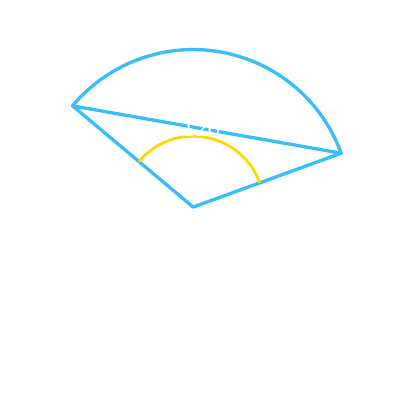
\begin{tikzpicture}[scale=1.0]
  \def\r{2.0}
  \def\a{20}
  \def\b{140}
  \coordinate (O) at (0,0);
  \coordinate (A) at (\a:\r);
  \coordinate (B) at (\b:\r);

  \draw[base] (O) circle (\r);
  \node[dot,label={[lab]below:$O$}] at (O) {};
  \node[dot,label={[lab]right:$A$}] at (A) {};
  \node[dot,label={[lab]left:$B$}] at (B) {};

  \draw[new] (O)--(A);
  \draw[new] (O)--(B);
  \draw[new] (A)--(B);
  \draw[new] (A) arc (\a:\b:\r);

  \pic[ang,"$120^\circ$",lab,angle radius=9mm,angle eccentricity=1.15] {angle=A--O--B};
\end{tikzpicture}
\end{StepDiagram}

\Step{2} Arc length:
\[
s=\frac{120}{360}\cdot 2\pi(6)=4\pi\ \text{cm}.
\]
\EqDiagram{$s=\dfrac{120}{360}\cdot 2\pi(6)=4\pi\ \text{cm}$}

\[
\boxed{4\pi\ \text{cm}}
\]
\end{QAPair}

% ============================================================
% Q7
\begin{QAPair}{Question 7}
\textcolor{gold}{\bfseries Question:} The diameter of a circle is $10$ cm and a chord parallel to it is $6$ cm long.
Find the distance between the chord and the diameter of the circle.
\tcblower
\textcolor{green}{\bfseries Answer:}\par

\Step{1} Diameter $10$ cm $\Rightarrow r=5$ cm. Chord length $L=6$ cm.
Drop perpendicular from centre to chord (it bisects chord).
\begin{StepDiagram}
\begin{tikzpicture}[scale=1.0]
  \def\r{2.2}
  \coordinate (O) at (0,0);
  \coordinate (A) at (-1.2,1.1);
  \coordinate (B) at ( 1.2,1.1);
  \coordinate (M) at (0,1.1);

  \draw[base] (O) circle (\r);
  \draw[help] (-\r,0)--(\r,0); % diameter line
  \node[dot,label={[lab]below:$O$}] at (O) {};

  \draw[new] (A)--(B); % chord
  \node[dot,label={[lab]above:$M$}] at (M) {};
  \draw[new] (O)--(M);
  \draw[base] ($(M)+(-0.18,0)$) -- ($(M)+(-0.18,-0.18)$) -- ($(M)+(0,-0.18)$);

  \node[lab] at (-0.55,1.35) {$3$};
  \node[lab] at ( 0.55,1.35) {$3$};
\end{tikzpicture}
\end{StepDiagram}

\Step{2} Distance from centre to chord:
\[
d=\sqrt{r^2-\left(\frac{L}{2}\right)^2}
=\sqrt{5^2-3^2}=\sqrt{16}=4\ \text{cm}.
\]
\EqDiagram{$d=\sqrt{25-9}=4\ \text{cm}$}

\Step{3} The diameter passes through the centre, so its distance from centre is $0$.
Hence distance between the chord and diameter is $d=4$ cm.
\EqDiagram{Distance (chord to diameter) $=4$ cm}

\[
\boxed{4\ \text{cm}}
\]
\end{QAPair}

% ============================================================
% Q8
\begin{QAPair}{Question 8}
\textcolor{gold}{\bfseries Question:} Find the area and perimeter of a semicircular window if its radius is $2.8$ feet.
\tcblower
\textcolor{green}{\bfseries Answer:}\par

\Step{1} Semicircle with radius $r=2.8$ ft.
\begin{StepDiagram}
\begin{tikzpicture}[scale=1.0]
  \def\r{2.2}
  \draw[base] (-\r,0) arc (180:0:\r);
  \draw[new] (-\r,0)--(\r,0); % diameter
  \node[lab] at (0,1.35) {curved edge};
  \node[lab] at (0,-0.25) {diameter};
\end{tikzpicture}
\end{StepDiagram}

\Step{2} Area:
\[
A=\frac12\pi r^2=\frac12\pi(2.8^2)=\frac{98}{25}\pi\ \text{ft}^2.
\]
\EqDiagram{$A=\dfrac{98}{25}\pi\ \text{ft}^2\ (\approx 12.32\ \text{ft}^2)$}

\Step{3} Perimeter (curved part + diameter):
\[
P=\pi r+2r=\pi(2.8)+5.6=\frac{14}{5}(\pi+2)\ \text{ft}.
\]
\EqDiagram{$P=\dfrac{14}{5}(\pi+2)\ \text{ft}\ (\approx 14.40\ \text{ft})$}

\[
\boxed{A=\frac{98}{25}\pi\ \text{ft}^2,\qquad P=\frac{14}{5}(\pi+2)\ \text{ft}}
\]
\end{QAPair}

% ============================================================
% Q9
\begin{QAPair}{Question 9}
\textcolor{gold}{\bfseries Question:} The building shown resembles a flying saucer. Find the length of supporting beam $AB$
if it makes an angle of $98^\circ$ with centre and the radius is $21$ m.
\tcblower
\textcolor{green}{\bfseries Answer:}\par

\Step{1} Beam $AB$ is a chord subtending central angle $\theta=98^\circ$ in a circle of radius $r=21$ m.
\begin{StepDiagram}
\begin{tikzpicture}[scale=1.0]
  \def\r{2.2}
  \def\a{41}
  \def\b{139}
  \coordinate (O) at (0,0);
  \coordinate (A) at (\a:\r);
  \coordinate (B) at (\b:\r);

  \draw[base] (O) circle (\r);
  \node[dot,label={[lab]below:$O$}] at (O) {};
  \node[dot,label={[lab]right:$A$}] at (A) {};
  \node[dot,label={[lab]left:$B$}] at (B) {};

  \draw[new] (O)--(A);
  \draw[new] (O)--(B);
  \draw[new] (A)--(B);

  \pic[ang,"$98^\circ$",lab,angle radius=9mm,angle eccentricity=1.15] {angle=A--O--B};
\end{tikzpicture}
\end{StepDiagram}

\Step{2} Chord length formula:
\[
AB=2r\sin\left(\frac{\theta}{2}\right)=2(21)\sin(49^\circ)=42\sin(49^\circ)\ \text{m}.
\]
\EqDiagram{$AB=42\sin(49^\circ)\ \text{m}\ (\approx 31.70\ \text{m})$}

\[
\boxed{AB=42\sin(49^\circ)\ \text{m}\approx 31.70\ \text{m}}
\]
\end{QAPair}

% ============================================================
% Q10
\begin{QAPair}{Question 10}
\textcolor{gold}{\bfseries Question:} A bridge is of semicircular shape with arc length $44$ m.
Find the length of the road constructed below.
\tcblower
\textcolor{green}{\bfseries Answer:}\par

\Step{1} For a semicircle, arc length $= \pi r$ (half of $2\pi r$).
\begin{StepDiagram}
\begin{tikzpicture}[scale=1.0]
  \def\r{2.2}
  \draw[base] (-\r,0) arc (180:0:\r);
  \draw[new] (-\r,0)--(\r,0);
  \node[lab] at (0,1.35) {arc $=44$ m};
  \node[lab] at (0,-0.25) {road (diameter)};
\end{tikzpicture}
\end{StepDiagram}

\Step{2} Solve for $r$:
\[
\pi r=44 \Rightarrow r=\frac{44}{\pi}.
\]
\EqDiagram{$r=\dfrac{44}{\pi}$}

\Step{3} Road length is the diameter:
\[
\text{Road}=2r=2\cdot \frac{44}{\pi}=\frac{88}{\pi}\ \text{m}.
\]
\EqDiagram{$\text{Road}=\dfrac{88}{\pi}\ \text{m}\ (\approx 28.01\ \text{m})$}

\[
\boxed{\frac{88}{\pi}\ \text{m}\approx 28.01\ \text{m}}
\]
\end{QAPair}

% ============================================================
% Q11
\begin{QAPair}{Question 11}
\textcolor{gold}{\bfseries Question:} Find the perimeter of lower portion (below the line $PQ$) of a circular window if: \\
radius $=2.1$ ft, $\angle POQ=105^\circ$, and shortest distance between centre $O$ and $PQ$ is $1.4$ ft. \\
Also find the area of upper portion (above $PQ$) of the window.
\tcblower
\textcolor{green}{\bfseries Answer:}\par

\Step{1} Draw chord $PQ$ at distance $OM=1.4$ ft from the centre ($M$ is midpoint of chord).
\begin{StepDiagram}
\begin{tikzpicture}[scale=1.0]
  \def\r{2.2}
  \coordinate (O) at (0,0);
  \coordinate (M) at (0,0.75);
  \coordinate (P) at (-1.55,0.75);
  \coordinate (Q) at ( 1.55,0.75);

  \draw[base] (O) circle (\r);
  \node[dot,label={[lab]below:$O$}] at (O) {};
  \draw[new] (P)--(Q);
  \node[dot,label={[lab]above:$M$}] at (M) {};
  \draw[new] (O)--(M);
  \draw[base] ($(M)+(-0.18,0)$) -- ($(M)+(-0.18,-0.18)$) -- ($(M)+(0,-0.18)$);

  \node[labm] at (0,-2.55) {Lower part = chord $PQ$ + \emph{major} arc};
\end{tikzpicture}
\end{StepDiagram}

\Step{2} Chord length using right triangle ($r=2.1$, $OM=1.4$):
\[
\frac{PQ}{2}=\sqrt{r^2-OM^2}=\sqrt{2.1^2-1.4^2}=\sqrt{2.45}=0.7\sqrt5,
\]
so
\[
PQ=1.4\sqrt5\ \text{ft}.
\]
\EqDiagram{$PQ=1.4\sqrt5\ \text{ft}\ (\approx 3.13\ \text{ft})$}

\Step{3} Major arc corresponds to $360^\circ-105^\circ=255^\circ$.
Major arc length:
\[
\ell_{\text{major}}=\frac{255}{360}\cdot 2\pi(2.1)=\frac{119}{40}\pi\ \text{ft}.
\]
\EqDiagram{$\ell_{\text{major}}=\dfrac{119}{40}\pi\ \text{ft}\ (\approx 9.35\ \text{ft})$}

\Step{4} Perimeter of lower portion:
\[
P_{\text{lower}}=PQ+\ell_{\text{major}}
=1.4\sqrt5+\frac{119}{40}\pi\ \text{ft}.
\]
\EqDiagram{$P_{\text{lower}}=1.4\sqrt5+\dfrac{119}{40}\pi\ \text{ft}\ (\approx 12.48\ \text{ft})$}

\Step{5} Area of upper portion (minor segment) for $\theta=105^\circ$:
\[
A_{\text{upper}}=A_{\text{sector}}-A_{\triangle}
=\frac{105}{360}\pi r^2-\frac12 r^2\sin 105^\circ.
\]
\EqDiagram{$A_{\text{upper}}=\dfrac{105}{360}\pi(2.1)^2-\dfrac12(2.1)^2\sin105^\circ$}

\Step{6} Substitute $r=\frac{21}{10}$:
\[
A_{\text{upper}}=\frac{1029}{800}\pi-\frac{441}{800}(\sqrt6+\sqrt2)\ \text{ft}^2.
\]
\EqDiagram{$A_{\text{upper}}=\dfrac{1029}{800}\pi-\dfrac{441}{800}(\sqrt6+\sqrt2)\ \text{ft}^2\ (\approx 1.91\ \text{ft}^2)$}

\[
\boxed{P_{\text{lower}}=1.4\sqrt5+\frac{119}{40}\pi\ \text{ft}}
\qquad
\boxed{A_{\text{upper}}=\frac{1029}{800}\pi-\frac{441}{800}(\sqrt6+\sqrt2)\ \text{ft}^2}
\]
\end{QAPair}

% ============================================================
% Q12
\begin{QAPair}{Question 12}
\textcolor{gold}{\bfseries Question:} A circular roller coaster is shown. Find the distance covered between two points making an angle of $80^\circ$ with the centre if its radius is $21$ ft.
\tcblower
\textcolor{green}{\bfseries Answer:}\par

\Step{1} The distance along the track is the arc length for $\theta=80^\circ$ and $r=21$ ft.
\begin{StepDiagram}
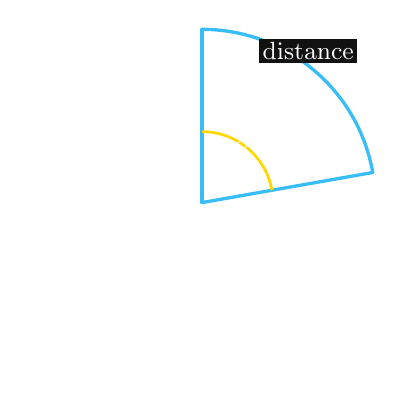
\begin{tikzpicture}[scale=1.0]
  \def\r{2.2}
  \def\a{10}
  \def\b{90}
  \coordinate (O) at (0,0);
  \coordinate (A) at (\a:\r);
  \coordinate (B) at (\b:\r);

  \draw[base] (O) circle (\r);
  \node[dot,label={[lab]below:$O$}] at (O) {};
  \draw[new] (O)--(A);
  \draw[new] (O)--(B);
  \draw[new] (A) arc (\a:\b:\r);
  \node[lab, fill=pairbg, inner sep=1.2pt] at (55:2.35) {distance};

  \pic[ang,"$80^\circ$",lab,angle radius=9mm,angle eccentricity=1.15] {angle=A--O--B};
\end{tikzpicture}
\end{StepDiagram}

\Step{2} Arc length:
\[
s=\frac{80}{360}\cdot 2\pi(21)=\frac{28}{3}\pi\ \text{ft}.
\]
\EqDiagram{$s=\dfrac{28}{3}\pi\ \text{ft}\ (\approx 29.32\ \text{ft})$}

\[
\boxed{\frac{28}{3}\pi\ \text{ft}\approx 29.32\ \text{ft}}
\]
\end{QAPair}

% ============================================================
% Q13
\begin{QAPair}{Question 13}
\textcolor{gold}{\bfseries Question:} The building shown is located in Guangzhou, China. The building's height is $138$ m and it has an empty circular core almost $59$ m in diameter. \\
(i) What is the covered area of the building? \\
(ii) Find the circular length of the part of building that touches ground if it makes an angle of $54^\circ$ with the centre.
\tcblower
\textcolor{green}{\bfseries Answer:}\par

\Step{1} Treat the face as an annulus (ring). Height $138$ m $\Rightarrow$ outer diameter $138$ m $\Rightarrow R=69$ m.
Core diameter $59$ m $\Rightarrow r=29.5$ m.
\begin{StepDiagram}
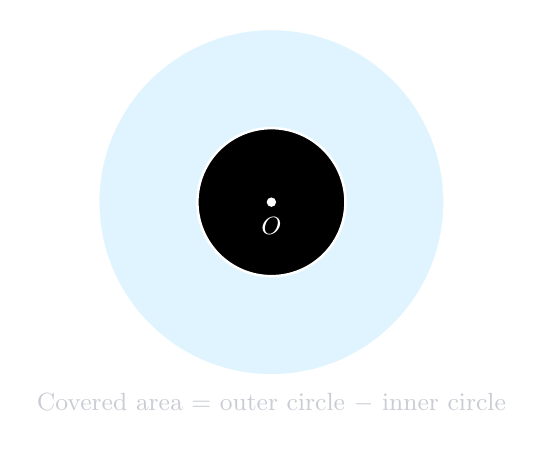
\begin{tikzpicture}[scale=1.0]
  \def\R{2.2}
  \def\r{0.94}
  \coordinate (O) at (0,0);
  \fill[cyan, opacity=0.16] (O) circle (\R);
  \fill[bg] (O) circle (\r);
  \draw[base] (O) circle (\R);
  \draw[base] (O) circle (\r);
  \node[dot,label={[lab]below:$O$}] at (O) {};
  \node[labm] at (0,-2.55) {Covered area = outer circle $-$ inner circle};
\end{tikzpicture}
\end{StepDiagram}

\Step{2} Covered area:
\[
A=\pi(R^2-r^2)=\pi(69^2-29.5^2).
\]
\EqDiagram{$A=\pi(69^2-29.5^2)=\dfrac{15563}{4}\pi\ \text{m}^2\ (\approx 12223.57\ \text{m}^2)$}

\Step{3} The part touching ground is an arc on the outer circle with $\theta=54^\circ$:
\[
\ell=\frac{54}{360}\cdot 2\pi(69)=\frac{207}{10}\pi\ \text{m}.
\]
\begin{StepDiagram}
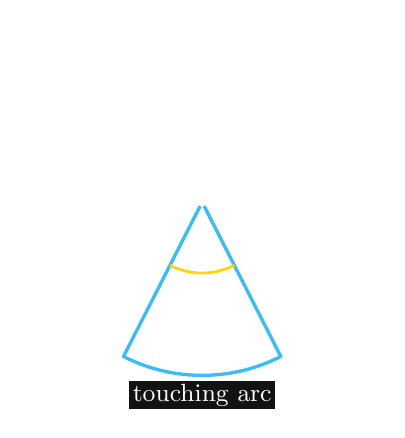
\begin{tikzpicture}[scale=1.0]
  \def\R{2.2}
  \def\a{-117}
  \def\b{-63}
  \coordinate (O) at (0,0);
  \coordinate (A) at (\a:\R);
  \coordinate (B) at (\b:\R);

  \draw[base] (O) circle (\R);
  \draw[new] (A) arc (\a:\b:\R); % ground-touch arc (illustrative)
  \draw[new] (O)--(A);
  \draw[new] (O)--(B);
  \node[dot,label={[lab]above:$O$}] at (O) {};
  \pic[ang,"$54^\circ$",lab,angle radius=9mm,angle eccentricity=1.15] {angle=A--O--B};
  \node[lab, fill=pairbg, inner sep=1.2pt] at (0,-2.45) {touching arc};
\end{tikzpicture}
\end{StepDiagram}

\Step{4} Final values:
\EqDiagram{$A=\dfrac{15563}{4}\pi\ \text{m}^2,\qquad \ell=\dfrac{207}{10}\pi\ \text{m}\ (\approx 65.03\ \text{m})$}

\[
\boxed{A=\frac{15563}{4}\pi\ \text{m}^2\approx 12223.57\ \text{m}^2}
\qquad
\boxed{\ell=\frac{207}{10}\pi\ \text{m}\approx 65.03\ \text{m}}
\]
\end{QAPair}

\end{document}
